\documentclass{article}
\usepackage{amsmath}
\usepackage{graphicx}
\usepackage{amsfonts}
\usepackage{amssymb}
\usepackage{geometry}
\geometry{letterpaper, portrait, margin=1in}
\usepackage{listings}

\title{ELCT 562 CA5: BER Performance Analysis of BPSK in AWGN Channel}
\author{Jacob Vaught \\ University of South Carolina}
\date{\today}

\begin{document}
\maketitle

\section{Introduction}
This document presents a simulation study of the bit error rate (BER) performance of Binary Phase-Shift Keying (BPSK) modulation over an Additive White Gaussian Noise (AWGN) channel. The analysis involves the development of a MATLAB simulation to encode random bit sequences, transmit them over an AWGN channel, and decode the received signals. The effectiveness of the receiver is evaluated by comparing the simulated BER against the theoretical BER.

\section{Theoretical Background}
\subsection{Binary Phase-Shift Keying (BPSK)}
BPSK is the simplest form of phase modulation that uses two phases to represent binary digits where typically, '0' and '1' are represented by signals \( s_0(t) = \sqrt{\frac{2E_b}{T}} cos(2\pi f_c t) \) and \( s_1(t) = \sqrt{\frac{2E_b}{T}} cos(2\pi f_c t + \pi) \) respectively.

\subsection{Additive White Gaussian Noise (AWGN)}
The AWGN channel adds white noise with a Gaussian distribution to the signal. The noise is characterized by its power spectral density \( N_0/2 \) and is added to the signal as \( r(t) = s(t) + n(t) \), where \( n(t) \) is the noise.

\subsection{Energy per Symbol to Noise Power Spectral Density Ratio (\(E_s/N_0\))}
The \( E_s/N_0 \) ratio is a measure of the signal strength relative to the noise level and is a key determinant of BER. Theoretical BER for BPSK in an AWGN channel is given by \( Q(\sqrt{2E_s/N_0}) \), where \( Q(x) \) is the Q-function.

\section{Code Explanation}
\subsection{Initialization}
The simulation begins with clearing the MATLAB environment to ensure no variables from previous runs affect the current simulation.

\subsection{Simulation Parameters}
The key parameters for the simulation include the roll-off factor (\( \rho \)), the sample rate (\( f_s \)), and the symbol spacing (\( T_s \)). These parameters define the shape of the transmitted signal and the quality of the sampling process.

\subsection{BER Simulation Loop}
A loop is constructed to simulate the transmission and reception of the signal over a range of \( E_s/N_0 \) values. For each value, a random bit sequence is generated, modulated into BPSK symbols, transmitted through the AWGN channel, and then processed by the receiver to estimate the original bit sequence.

\subsection{Receiver Function}
The receiver function processes the received IQ data using a matched filter and then samples the filter output to estimate the transmitted symbols.

\subsection{Waveform Generation}
The waveform generation involves up-sampling the BPSK symbols and then shaping them with a root-raised cosine filter to limit the bandwidth and reduce intersymbol interference.

\subsection{Root-Raised Cosine (RRC) Filter}
The RRC filter is defined by its roll-off factor and is used to shape the transmitted signal and to perform matched filtering at the receiver.

\section{Results Discussion}
\subsection{BER Performance}
The BER performance graph shows the simulated BER as a function of \( E_s/N_0 \) alongside the theoretical BER curve. As expected, the BER decreases with an increase in \( E_s/N_0 \).

\begin{figure}[ht]
\centering
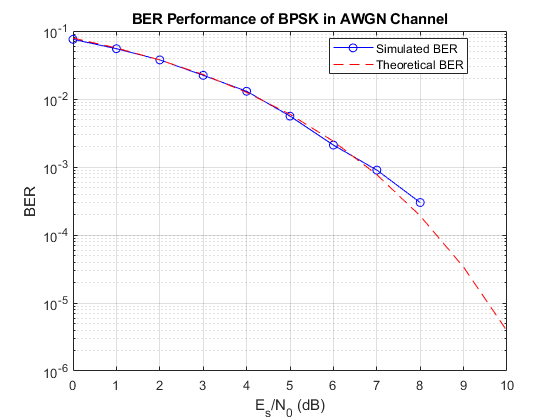
\includegraphics[width=0.8\textwidth]{BER.png}
\caption{BER Performance of BPSK in AWGN Channel.}
\end{figure}

\subsection{Transmit Filter}
The transmit filter's impulse response defines the shape of each transmitted symbol and thus affects the bandwidth and the resistance to intersymbol interference.

\begin{figure}[ht]
\centering
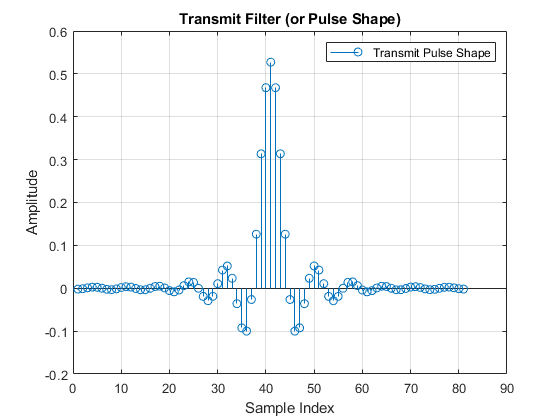
\includegraphics[width=0.8\textwidth]{filter.png}
\caption{Transmit Filter (or Pulse Shape).}
\end{figure}

\subsection{Signal in Time}
The time-domain representation of the in-phase component of the signal demonstrates how the RRC filter shapes the BPSK symbols.

\begin{figure}[ht]
\centering
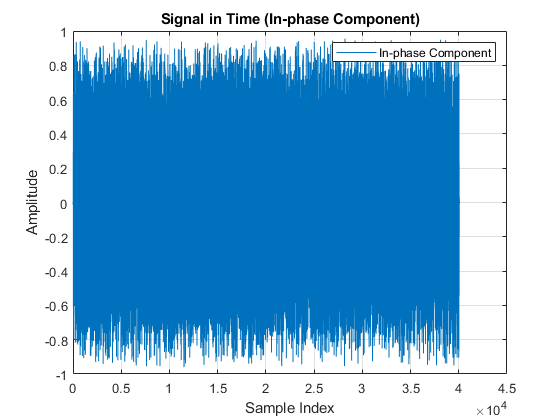
\includegraphics[width=0.8\textwidth]{waveform.png}
\caption{Signal in Time (In-phase Component).}
\end{figure}
The figure above represents the in-phase component of the transmitted signal in the time domain. It illustrates the effect of the root-raised cosine (RRC) filter on the signal shape and how it influences the overall bandwidth and time-domain representation of the BPSK modulated signal. The discrete nature of the signal can also be observed, which is a result of the sampling process and the subsequent digital-to-analog conversion in a practical communication system.

\section{Conclusion}
The MATLAB simulation developed for this study effectively demonstrates the BER performance of BPSK modulation in an AWGN channel. The comparison between the simulated BER and the theoretical BER confirms the accuracy of the simulation. The results obtained reinforce the theoretical expectations, showing a decrease in BER with an increase in \(E_s/N_0\). The analysis performed provides valuable insights into the design and performance evaluation of digital communication systems.

\appendix
\section{MATLAB Code}
The MATLAB code used for the simulation is provided below. It includes initialization, parameter definition, BER simulation loop, receiver function, waveform generation, and the RRC filter function.

\lstset{basicstyle=\ttfamily, breaklines=true, frame=single}
\begin{lstlisting}[language=Matlab]
%% Initialization
clear all; close all; clc;  % Clear environment, close figures, clear command window

% Design and simulation parameters
rho = 0.2; % RRC roll-off factor
fsample = 2e9; % Sample rate: 2 GHz
Tsample = 1/fsample; % Sample period
Tspacing = 2e-9; % Symbol spacing: 2 ns
EsN0dBlist = 0:10; % Es/N0 range in dB
N = 10000; % Number of bits for simulation
Nover = Tspacing/Tsample; % Oversampling factor

%%%%%%%%%%%%%%%%%%%%%%%%%HOMEWORK%%%%%%%%%%%%%%%%%%%%%%%%%%%%%%%%%%%%%%%%%
%% Simulation Setup
% Initialize error list
numberOfErrorsList = zeros(size(EsN0dBlist));

%% BER Simulation Loop
for indEsN0dB = 1:length(EsN0dBlist)
    % Generate random bits and corresponding IQ data
    bitsTX = randi([0, 1], N, 1); % Random bits
    symbolsTX = 2*bitsTX - 1; % BPSK modulation
    [IQdataTX, pTX] = myWaveform(rho, symbolsTX, Tsample, Tspacing);
    
    % Channel simulation: Add AWGN
    EsN0 = 10^(EsN0dBlist(indEsN0dB)/10); % Linear scale Es/N0
    N0 = 1/EsN0; % Noise spectral density
    noiseVariance = N0/2;
    noise = sqrt(noiseVariance) * (randn(size(IQdataTX)) + 1i * randn(size(IQdataTX)));
    IQdataRX = IQdataTX + noise; % Received signal
    
    % Decode received signal
    symbolsRX = myReceiver(IQdataRX, pTX, Nover, N);
    
    % Count errors
    errors = sum(bitsTX ~= symbolsRX);
    numberOfErrorsList(indEsN0dB) = errors;
end

%% Calculate and Plot BER
BERlist = numberOfErrorsList / N; % BER calculation
BERlistTheory = qfunc(sqrt(2 * 10.^(EsN0dBlist / 10))); % Theoretical BER

% Plotting BER Performance
figure;
semilogy(EsN0dBlist, BERlist, 'b-o', 'DisplayName', 'Simulated BER');
hold on;
semilogy(EsN0dBlist, BERlistTheory, 'r--', 'DisplayName', 'Theoretical BER');
xlabel('E_s/N_0 (dB)');
ylabel('BER');
title('BER Performance of BPSK in AWGN Channel');
legend('Location', 'best');
grid on;

figure(2);
plot(real(IQdataTX), 'DisplayName', 'In-phase Component');
title('Signal in Time (In-phase Component)');
xlabel('Sample Index');
ylabel('Amplitude');
legend show;
grid on;

figure(3);
stem(pTX, 'DisplayName', 'Transmit Pulse Shape');
title('Transmit Filter (or Pulse Shape)');
xlabel('Sample Index');
ylabel('Amplitude');
legend show;
grid on;

function [symbolsRX] = myReceiver(IQdata, prx, Nover, symbolsLength)
    rxFiltered = conv(IQdata, conj(fliplr(prx)), 'same');
    filterDelay = (length(prx) - 1) / 2;
    startIndex = 1 + filterDelay; % Adjust this based on the actual delay
    symbolsRX = rxFiltered(startIndex:Nover:startIndex+Nover*(symbolsLength-1));
    symbolsRX = real(symbolsRX) > 0; % Convert to bits (0 or 1)
end
%%%%%%%%%%%%%%%%%%%%%%%%%HOMEWORK%%%%%%%%%%%%%%%%%%%%%%%%%%%%%%%%%%%%%%%%%


function [IQdata ptx] =  myWaveform(rho, symbols, Tsample, Tspacing)
    Nover = Tspacing/Tsample;
    n = [-10:1/Nover:10];
    h = rrc(rho,n); 
    h = h/sqrt(sum(abs(h).^2));
    symbolsUp = upsample(symbols,Nover);
    IQdata = conv(h,symbolsUp);
    ptx = h;
end
function h = rrc(beta,t)
    h = (sin((1-beta)*pi*t)+4*beta*t.*cos((1+beta)*pi*t))./ (pi*t.*(1-(4*beta*t).^2));
    h(t==0) = 1 - beta*(1 - (4/pi));
    h(t == 1/4/beta | t == -1/4/beta) = beta/sqrt(2)*((1+2/pi) * sin(pi/(4*beta)) + (1-2/pi) * cos(pi/(4*beta)));
end


\end{lstlisting}

\end{document}
